%%%%%%%%%%%%%%%%%%%%%%%%%%%%%%%%%%%%%%%%%
% University/School Laboratory Report
% LaTeX Template
% Version 3.1 (25/3/14)
%
% This template has been downloaded from:
% http://www.LaTeXTemplates.com
%
% Original author:
% Linux and Unix Users Group at Virginia Tech Wiki 
% (https://vtluug.org/wiki/Example_LaTeX_chem_lab_report)
%
% License:
% CC BY-NC-SA 3.0 (http://creativecommons.org/licenses/by-nc-sa/3.0/)
%
%%%%%%%%%%%%%%%%%%%%%%%%%%%%%%%%%%%%%%%%%

%----------------------------------------------------------------------------------------
%	PACKAGES AND DOCUMENT CONFIGURATIONS
%----------------------------------------------------------------------------------------

\documentclass{article}

\usepackage[version=3]{mhchem} % Package for chemical equation typesetting
\usepackage{siunitx} % Provides the \SI{}{} and \si{} command for typesetting SI units
\usepackage{graphicx} % Required for the inclusion of images
\usepackage{natbib} % Required to change bibliography style to APA
\usepackage{amsmath} % Required for some math elements 

\setlength\parindent{0pt} % Removes all indentation from paragraphs

\renewcommand{\labelenumi}{\alph{enumi}.} % Make numbering in the enumerate environment by letter rather than number (e.g. section 6)

%\usepackage{times} % Uncomment to use the Times New Roman font

%----------------------------------------------------------------------------------------
%	DOCUMENT INFORMATION
%----------------------------------------------------------------------------------------

\title{Connettore Publish-Subscribe Content-Based adeguato ad ambiente Mobile per mezzo di politiche adattative } % Title

\author{Stefano \textsc{Agostini} Matricola: 0234240 \\ Paolo \textsc{Salom\'e} Matricola: 0233502 \\ Alessandro \textsc{Valenti} Matricola: 0228709} % Author name

\date{\today} % Date for the report

\begin{document}

\maketitle % Insert the title, author and date

%\begin{center}
%\begin{tabular}{l r}
%Date Performed: & January 1, 2012 \\ % Date the experiment was performed
%Partners: & James Smith \\ % Partner names
%& Mary Smith \\
%Instructor: & Professor Smith % Instructor/supervisor
%\end{tabular}
%\end{center}

% If you wish to include an abstract, uncomment the lines below
% \begin{abstract}
% Abstract text
% \end{abstract}

%----------------------------------------------------------------------------------------
%	SECTION 1
%----------------------------------------------------------------------------------------

\section{Introduzione}

Il connettore \textit{Publish-Subscribe} presenta caratteristiche interessanti per sistemi caratterizzati da una elevata dinamicit\'a, grazie all'elevato livello di disaccoppiamento che \'e in grado di garantire tra componenti. I componenti coinvolti nell'interazione, per mezzo del connettore, sono i \textit{produttori} e i \textit{consumatori} di determinati eventi generabili. Un evento \'e caratterizzato dal cosidetto \textit{topic} che rappresenta il suo argomento d'appartenenza al quale un \textit{consumatore} pu\'o sottoscriversi se interessato a tale classe di informazioni; il \textit{produttore} a sua volta pu\'o pubblicare eventi associati ad un determinato \textit{topic}. Nello specifico \'e possibile caratterizzare un determinato evento (dopo averlo associato ad un \textit{topic}) in base al suo contenuto utilizzando la politica del tipo \textit{content-based}. Tale modalit\'a di sottoscrizione viene realizzata specificando un filtro e di conseguenza favorisce la riduzione del carico di eventi recapitati ai \textit{consumatori}. Il connettore realizzato si presta all'utilizzo in ambiente mobile in quanto assicura un alto grado di disaccoppiamento, continuando a garantire uno scambio affidabile di messaggi tra le entit\'a coinvolte. Tuttavia ci siamo posti come obiettivo quello di aggiungere a tale sistema politiche adattative che tengano conto delle limitate risorse energetiche e computazionali a disposizione dei nodi mobili, continuando a garantire uno scambio affidabile di messaggi tra le entit\'a attraverso il connettore.
Intuendo un relazione funzionale tra consumo energetico e traffico generato dal nodo mobile, abbiamo compiuto uno studio statistico per avallare la nostra ipotesi che si \'e rivelato soddisfacente: pertanto abbiamo potuto realizzare un modello matematico finale. 
La nostra politica adattativa ci permette di controllare il tasso di consumo energetico controllando direttamente la frequenza di interazione del nodo mobile con la rete, gestendo, tramite un monitoraggio continuo dello stato della batteria, le risorse limitate del dispositivo. % scrivere in una frase che il nostro sistema implementa mape?

\section{Obiettivi}

L'obiettivo \'e quello di realizzare un connettore \textit{Publish-Subscribe} in modalit\'a \textit{content-based} (basato su \textit{string pattern matching}) ed adattarlo ad ambiente mobile. Nel dettaglio il nostro sistema deve essere costituito da nodi mobili che possono assumere il ruolo di \textit{consumatore o produttore} e dal connettore che deve comporsi delle seguenti entit\'a:

\begin{itemize}
\item{\textit{Event-Service}, il quale si preoccupa di gestire gli eventi generati e di recapitare notifiche}
\item{\textit{Filter-Service}, il quale realizza la modalit\'a di sottoscrizione \textit{content-based}}
\end{itemize}

Si vuole inoltre adattare tale sistema ad ambiente mobile mediante una politica che abbia come scopo quello di monitorare e controllare:

\begin{itemize}
\item{\textit{Il consumo energetico}}
\item{\textit{Il traffico generato} nell'interazione tra nodo mobile e connettore}
\end{itemize}

\section{Architettura generale}

Il sistema si basa fondamentalmente su un'architettura centralizzata. Infatti il connettore \textit{Publish-Subscribe} si compone di un server che svolge sia la funzione di \textit{Event-Service} che la funzione di \textit{Filter-Service}. I client non interagiscono direttamente con il connettore ma scambiano messaggi mediante delle code che implementano il paradigma di interazione \textit{message queueing}. Tale paradigma offre dei vantaggi in termini di disaccoppiamento spaziale e temporale, garantendo la possibilit\'a al client di potersi disattivare o spegnere immantinentemente una volta inoltrato un messaggio.
\\
Il server gestisce, tramite una \textit{database non relazionale} distribuito, la persistenza delle informazioni indispensabili per il corretto funzionamento del sistema dal punto di vista dei client, ovvero

\begin{itemize}
\item{\textit{Topic}}
\item{\textit{Sottoscrizioni e Filtri}}
\end{itemize}

I nodi mobili, cos\'i come il server, gestiscono la persistenza in locale di alcune informazioni attraverso un \textit{database relazionale}. Tali informazioni sono i \textit{topic} al momento disponibili nel sistema, le \textit{notifiche} in ingresso, le \textit{sottoscrizioni} effettuate con i relativi \textit{topic e filtri}. Il client attraverso procedure interne effettua, periodicamente,  un'operazione di \textit{pull} sulla coda per poter aggiornare i dati relativi alle notifiche ad esso destinate. Analogamente richiede al server la lista dei \textit{topic} disponibili per aggiornare le sue informazioni locali. Tutto ci\'o viene attuato per promuovere un utilizzo offline dell'applicazione in caso di disconnessione, scenario possibile nell'ambito dei sistemi mobili.\\
Di seguito illustriamo l'architettura attraverso uno schema in \figurename{~\ref{fig:Architettura}}.

\begin{figure}[h]
\begin{center}
\centering
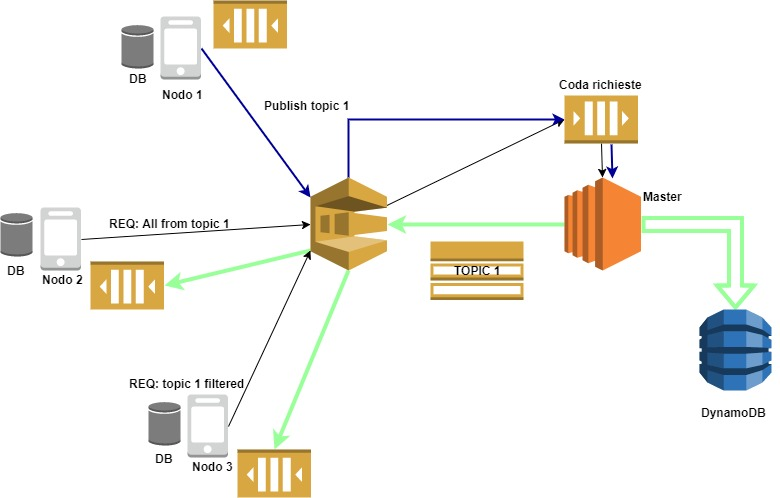
\includegraphics[width=1.25\textwidth]{architettura.jpg} % Include the image placeholder.png
\caption{Architettura}
\label{fig:Architettura}
\end{center}
\end{figure}

\subsection{Servizi Cloud}

Come \textit{Cloud Provider} \'e stato scelto \textit{Amazon AWS}. I servizi utilizzati per l'implementazione del connettore sono:

\begin{itemize}
\item{\textbf{Amazon EC2}: servizio \textit{IaaS} sfruttato per la realizzazione del nodo master che identifica il server dell'architettura. Svolge il ruolo di \textit{Event-Service e Filter-Service} nonch\'e di gestore del \textit{database NoSQL}. Per la comunicazione con i nodi client interagisce con le code del servizio \textit{Amazon SQS}}
\item{\textbf{Amazon SQS}: \'e un servizio di accodamento di messaggi distribuito che disaccoppia completamente i componenti dell'architettura. In tal modo semplifica e riduce i costi del coordinamento dei componenti stessi. Offre un \textit{throughput} elevato e \textit{tunable}, un ordinamento semplificato e distribuzione di tipo \textit{at-least-once}. In generale \'e possibile impostare un algoritmo di \textit{scheduling} dei messaggi: nel nostro caso \'e stato utilizzato l'algoritmo \textit{FIFO}}
\item{\textbf{Amazon DynamoDB}: \'e un servizio di \textit{datastorage} distribuito basato su un \textit{database NoSQL} di tipo \textit{key-value}. \textit{DynamoDB} implementa un sistema di tipo \textit{AP}, disponibilit\'a e tolleranza alle partizioni dei dati, secondo il \textit{CAP Theorem}. L'alto grado di disponibilit\'a ed un accesso di tipo \textit{anywhere} alle informazioni sono due caratteristiche adatte ad un utilizzo in ambiente mobile. Essendo inoltre un database \textit{read-mostly}, ovvero pensato prevalentemente per operazioni di lettura, si adatta perfettamente al nostro sistema, il quale richiede pi\'u letture che scritture.}
\end{itemize}

\subsection{Ambiente Client}
Il nostro sistema \'e pensato per un utilizzo da parte di \textit{client leggeri} con sistema operativo \textit{Android}. \textit{Android} \'e un sistema operativo per dispositivi mobili sviluppato da \textit{Google Inc.} e basato sul kernel \textit{Linux}. Le applicazioni che vengono eseguite sulle piattaforme \textit{Android} sono scritte prevalentemente in linguaggio \textit{Java}, come nel nostro caso. L'applicazione \textit{client} interagisce con un \textit{database relazionale} interno di tipo \textit{SQLite}.

\subsection{Ambiente Server}
Sfruttando il servizio \textit{IaaS di Amazon EC2}, \'e stato possibile scegliere il sistema operativo del server e le caratteristiche della macchina \textit{host}. In particolare abbiamo scelto un'istanza \textit{t2.micro} dotata di una \textit{virtual cpu}, \textit{1 GB di ram} e \textit{8 GB di storage}. \'E stato scelto come sistema operativo \textit{Linux Ubuntu Server v.16.04 LTS}. La scelta di tale sistema operativo \'e da ricondurre alla semplicit\'a di installazione di componenti aggiuntivi e alla sua versatilit\'a.

\subsection{Interazione dei componenti}
Per promuovere la comunicazione tra i client ed il server, disaccoppiandoli, \'e stato scelto di utilizzare diverse code \textit{SQS}, partizionandone i compiti. In particolare vengono generate tre code fisse per richiedere l'esecuzione delle operazioni fondamentali di un sistema \textit{Publish-Subscribe} al  server:

\begin{itemize}
\item{\textbf{Creation Queue}: i client scrivono su questa coda per richiedere al server la creazione di un determinato \textit{topic}}
\item{\textbf{Notification Queue}: i client scrivono su questa coda per pubblicare una notifica su un determinato \textit{topic}}
\item{\textbf{Subscription Queue}: i client scrivono su questa coda per sottoscriversi in modalit\'a \textit{content-based} ad un determinato \textit{topic} oppure annullare una sottoscrizione precedentemente effettuata}
\end{itemize}

Ogni messaggio proveniente dai nodi mobili raggiunge il server per mezzo delle tre code fisse sopra descritte (come si nota in \figurename{~\ref{fig:Architettura}}). Il server elabora i messaggi in ingresso ed aggiorna le informazioni riguardanti i \textit{topic} e le sottoscrizioni nell'istanza di \textit{DynamoDB}.
\\
Per la ricezione di messaggi ogni client ha a disposizione una coda dedicata, la quale viene creata al momento dell'ingresso del nodo nel sistema ed \'e utilizzata per la ricezione dei messaggi di notifica.
\\
Infine il database \textit{SQLite}, presente in ogni client, \'e utilizzato per tenere traccia dei \textit{topic} presenti al momento nell'istanza di \textit{DynamoDB} e per memorizzare le notifiche ricevute.

\section{Implementazione}

\subsection{Server}
Abbiamo scelto di utilizzare lato server la piattaforma \textit{event-driven Node.js} per motivi di immediatezza, versatilit\'a  ed efficienza. Tale piattaforma supporta il linguaggio di programmazione \textit{Javascript}, linguaggio di scripting orientato agli oggetti e agli eventi. L'efficienza di \textit{Node.js} \'e legata al suo modello di \textit{networking}, ossia \textit{I/O event-driven}. La piattaforma richiede al sistema operativo di ricevere notifiche al verificarsi di determinati eventi e rimane in modalit\'a \textit{sleep} fino alla ricezione della notifica stessa, in corrispondenza della quale avvia l'esecuzione di una funzione di \textit{callback} di risposta. Tale modello di \textit{networking} si rivela efficiente nella gestione di un elevato traffico di rete, come potrebbe accadere nel caso del nostro sistema.
\\
Di seguito ci apprestiamo a descrivere puntualmente l'implementazione dei componenti server.

\subsubsection{Formato \textit{JSON} dei messaggi scambiati}

I messaggi diretti da client a server possono essere di tre tipi (un tipo per coda):

\begin{itemize}

\item{\textbf{Crezione-rimozione di un topic}:}

\begin{tabular}{ll}
\{\\
	   \hspace{10mm} "type": string, // "CREATE" or "DELETE"\\
              \hspace{10mm} "userID": string, // macaddress\\
              \hspace{10mm} "topicName": string
\\
\}
\end{tabular}

\item{\textbf{Sottoscrizione-Cancellazione}:}

\begin{tabular}{ll}
\{\\	   
            \hspace{10mm} "type": string, // "SUB" or "UNSUB" or "UNSUBALL"\\
            \hspace{10mm} "userID": string, // macaddress\\
            \hspace{10mm} "topicName": string,\\
            \hspace{10mm} "filter": string 
\\
\}
\end{tabular}

\item{\textbf{Pubblicazione di notifiche}:}

\begin{tabular}{ll}
\{\\	   
           \hspace{10mm} "userID": string, // macaddress\\
           \hspace{10mm} "topicName": string,\\
           \hspace{10mm} "messageBody": string
\\
\}
\end{tabular}

\end{itemize}

I messaggi di notifica elaborati dal server e destinati alle code dedicate dei client hanno il seguente formato:

\begin{tabular}{ll}
\{\\	   
           \hspace{10mm} "topicName": string, \\
           \hspace{10mm} "messageBody": string
\\
\}
\end{tabular}

\subsubsection{AWS SDK}
\textit{Amazon AWS} mette a disposizione delle librerie ai programmatori per consentirgli di interagire e accedere ai servizi \textit{Cloud} da codice. In particolare \textit{AWS} supporta anche \textit{Javascript} con le proprie \textit{SDK} (\textit{Software Development Kit}). Sono state utilizzate le \textit{API AWS SDK} relative ai servizi \textit{SQS e DynamoDB} ed estese per mezzo di due librerie: \textit{sqs\_api.js e dynamo\_api.js}.\\

\textbf{sqs\_api.js}
\begin{itemize}
\item{\textit{create\_queue}: crea una coda identificata dall'attributo \textit{QueueNamePrefix} (parametro della funzione) se non esiste. Questa funzione viene utilizzata sia per la creazione delle tre code fisse che di quelle dedicate ai singoli nodi client.}
\item{\textit{write\_queue}: scrive un messaggio nella coda specificata (messaggio e nome della coda entrambi parametri della funzione). Per risalire alla coda, ricava il suo \textit{URL} mediante l'\textit{API SDK getQueueUrl} utilizzando il suo nome. Se il recupero va a buon fine, viene inviato il messaggio sulla coda invocando \textit{l'API SDK sendMessage}.}
\item{\textit{read\_queue}: legge i messaggi presenti nella coda di cui \'e specificato il nome (parametro della funzione). Ricava lo \textit{URL} della coda mediante l'\textit{API SDK getQueueUrl} alla quale passa il nome come argomento. Se la \textit{getQueueUrl} va a buon fine, vengono recuperati i messaggi presenti nella coda selezionata grazie all'\textit{API SDK receiveMessage}. Nella \textit{callback} della \textit{receiveMessage} viene generato un nuovo processo che resta in attesa della comunicazione dei messaggi da parte del processo padre. Quest'ultimo invia i messaggi letti dalla coda al processo figlio sfruttando la funzione \textit{send} dell'\textit{IPC di Node.js}.  In ricezione, il processo figlio (definito come \textit{consumer}, i cui dettagli sono nella sezione 4.1.4) elabora i messaggi e termina. Tutti i messaggi letti dalla coda vengono eliminati dalla stessa attraverso la funzione \textit{delete\_messages} che ci apprestiamo a descrivere.}
\item{\textit{delete\_messages}: prende come parametri lo \textit{URL} della coda e la lista delle \textit{entries} lette, oggetti che seguono un formato specificato dagli standard \textit{AWS SDK}. Per l'eliminazione viene invocata l'\textit{API SDK deleteMessageBatch}, la quale permette la cancellazione di \textit{batch} interi di messaggi.}
\end{itemize}

\textbf{dynamo\_api.js}
\begin{itemize}
\item{\textit{creation\_table}: prende come parametro il nome della tabella da creare (supporta la creazione delle tabelle \textit{Topic e Subscription}). Definisce il formato della tabella per la sua creazione per mezzo dell'\textit{API SDK createTable}. La tabella \textit{Topic} ha come chiave il \textit{topicName} (\textit{string}) che ricopre il ruolo di \textit{partition key}. Invece la tabella \textit{Subscription} ha come chiave la coppia \textit{(topicName, userID)} (entrambe stringhe) e la prima ha il ruolo di \textit{partition key} mentre la seconda quello di \textit{sort key}.}
\item{\textit{create\_topic}: prende come parametri il \textit{topicName} e lo \textit{user\_id} (creatore del \textit{topic}). Utilizza l'\textit{API SDK get} e, se il \textit{topic} non \'e presente nella tabella \textit{Topic}, crea un nuovo \textit{item} e lo salva usando l'\textit{API SDK put}.}
\item{\textit{delete\_topic}: prende come parametri il \textit{topic\_name} e lo \textit{user\_id} (identificativo del client che ha richiesto al server di rimuovere il \textit{topic}). Recupera, mediante l'\textit{API SDK get}, il \textit{topic} dalla tabella e controlla se l'\textit{id} del creatore coincide con l'\textit{id} del client richiedente. In caso affermativo rimuove l'\textit{item} dalla tabella usando l'\textit{API SDK delete}.}
\item{\textit{create\_subscription}: prende come parametri \textit{topic\_name, user\_id} e \textit{filter}. Controlla l'esistenza del \textit{topic} nella tabella \textit{Topic}. Se \'e verificata scrive nella tabella \textit{Subscription} il nuovo \textit{item}, con chiave \textit{(topic\_name, user\_id)}.}
\item{\textit{delete\_subscription}: prende come parametri \textit{topic\_name} e \textit{user\_id}. Effettua la cancellazione dalla tabella \textit{Subscription} dell'\textit{item} con chiave \textit{(topic\_name, user\_id)}, usando l'\textit{API SDK delete}.}
\item{\textit{scan\_all\_topics}: utilizza l'\textit{API SDK scan} per estrarre la lista dei \textit{topic} al momento presenti nel sistema.}
\item{\textit{send\_notification}: prende come parametri \textit{topic\_name} e \textit{message\_body} (rispettivamente il \textit{topic} e il messaggio inviato dal client che vuole effettuare una \textit{publish} su di esso). Effettua una \textit{query} sulla tabella \textit{Subscription}, tramite l'\textit{API SDK query}, specificando il \textit{topic\_name}. Il risultato delle \textit{query} \'e una lista di coppie \textit{(user\_id, filter)}, ognuna delle quali rappresenta un sottoscritto al \textit{topic} ed il relativo filtro. Per ogni \textit{item} della lista viene controllata l'occorrenza del suo filtro all'interno del \textit{message\_body}, ed in caso fosse verificata viene inoltrata la notifica alla coda dedicata del client mediante la funzione \textit{write\_queue} della libreria \textit{sqs\_api.js}.}
\end{itemize}

\subsubsection{\textit{Readers}}
I tre processi \textit{Readers} si occupano di leggere periodicamente dalle tre code fisse \textit{Creation Queue}, \textit{Notification Queue} e \textit{Subscription Queue}. Tali processi sono continuamente in esecuzione e sfruttano la funzione \textit{polling} del modulo \textit{polling.js}, la quale legge periodicamente dalla coda specificata, passata come argomento, mediante la funzione \textit{read\_queue} della libreria \textit{sqs\_api}. Nel caso in esame \'e stato scelto come intervallo di lettura un tempo pari a \textit{5000 millisec}.

\subsubsection{\textit{Consumer e Updaters}}
\textit{Consumer} \'e un processo che ha il compito di catalogare e gestire i messaggi in funzione della coda dalla quale sono stati letti: implementa nella pratica uno \textit{switch-case}. 


\subsubsection{\textit{Server Http e Routes}}

\subsubsection{\textit{Main}}

\subsection{Client}
 
%----------------------------------------------------------------------------------------
%	SECTION 2
%----------------------------------------------------------------------------------------

\section{Experimental Data}

\begin{tabular}{ll}
Mass of empty crucible & \SI{7.28}{\gram}\\
Mass of crucible and magnesium before heating & \SI{8.59}{\gram}\\
Mass of crucible and magnesium oxide after heating & \SI{9.46}{\gram}\\
Balance used & \#4\\
Magnesium from sample bottle & \#1
\end{tabular}

%----------------------------------------------------------------------------------------
%	SECTION 3
%----------------------------------------------------------------------------------------

\section{Sample Calculation}

\begin{tabular}{ll}
%Mass of magnesium metal & = \SI{8.59}{\gram} - \SI{7.28}{\gram}\\
%& = \SI{1.31}{\gram}\\
%Mass of magnesium oxide & = \SI{9.46}{\gram} - \SI{7.28}{\gram}\\
%& = \SI{2.18}{\gram}\\
%Mass of oxygen & = \SI{2.18}{\gram} - \SI{1.31}{\gram}\\
%& = \SI{0.87}{\gram}
\end{tabular}

Because of this reaction, the required ratio is the atomic weight of magnesium: \SI{16.00}{\gram} of oxygen as experimental mass of Mg: experimental mass of oxygen or $\frac{x}{1.31}=\frac{16}{0.87}$ from which, $M_{\ce{Mg}} = 16.00 \times \frac{1.31}{0.87} = 24.1 = \SI{24}{\gram\per\mole}$ (to two significant figures).

%----------------------------------------------------------------------------------------
%	SECTION 4
%----------------------------------------------------------------------------------------

\section{Results and Conclusions}

The atomic weight of magnesium is concluded to be \SI{24}{\gram\per\mol}, as determined by the stoichiometry of its chemical combination with oxygen. This result is in agreement with the accepted value.

\begin{figure}[h]
\begin{center}

\includegraphics[width=0.65\textwidth]{placeholder} % Include the image placeholder.png
\caption{Figure caption.}
\end{center}
\end{figure}

%----------------------------------------------------------------------------------------
%	SECTION 5
%----------------------------------------------------------------------------------------

\section{Discussion of Experimental Uncertainty}

The accepted value (periodic table) is \SI{24.3}{\gram\per\mole} \cite{Smith:2012qr}. The percentage discrepancy between the accepted value and the result obtained here is 1.3\%. Because only a single measurement was made, it is not possible to calculate an estimated standard deviation.

The most obvious source of experimental uncertainty is the limited precision of the balance. Other potential sources of experimental uncertainty are: the reaction might not be complete; if not enough time was allowed for total oxidation, less than complete oxidation of the magnesium might have, in part, reacted with nitrogen in the air (incorrect reaction); the magnesium oxide might have absorbed water from the air, and thus weigh ``too much." Because the result obtained is close to the accepted value it is possible that some of these experimental uncertainties have fortuitously cancelled one another.

%----------------------------------------------------------------------------------------
%	SECTION 6
%----------------------------------------------------------------------------------------

\section{Answers to Definitions}

\begin{enumerate}
\begin{item}
The \emph{atomic weight of an element} is the relative weight of one of its atoms compared to C-12 with a weight of 12.0000000$\ldots$, hydrogen with a weight of 1.008, to oxygen with a weight of 16.00. Atomic weight is also the average weight of all the atoms of that element as they occur in nature.
\end{item}
\begin{item}
The \emph{units of atomic weight} are two-fold, with an identical numerical value. They are g/mole of atoms (or just g/mol) or amu/atom.
\end{item}
\begin{item}
\emph{Percentage discrepancy} between an accepted (literature) value and an experimental value is
\begin{equation*}
\frac{\mathrm{experimental\;result} - \mathrm{accepted\;result}}{\mathrm{accepted\;result}}
\end{equation*}
\end{item}
\end{enumerate}

%----------------------------------------------------------------------------------------
%	BIBLIOGRAPHY
%----------------------------------------------------------------------------------------

\bibliographystyle{apalike}

\bibliography{sample}

%----------------------------------------------------------------------------------------


\end{document}